\begin{figure}[H]
  \centering
  
  \begin{subfigure}[b]{0.5\textwidth}
  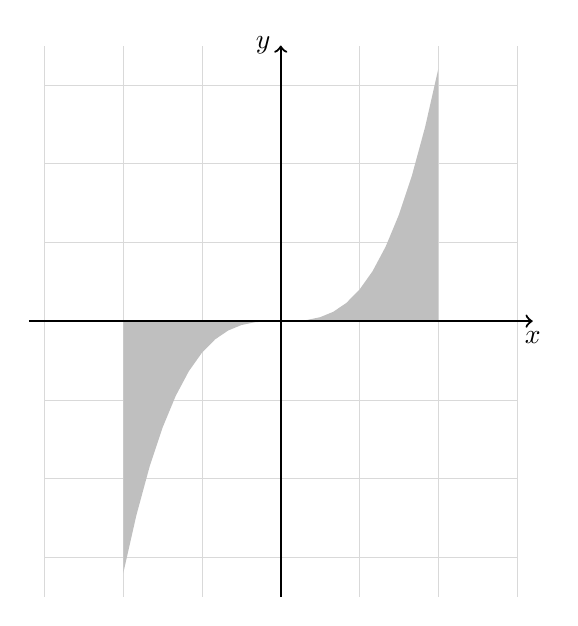
\begin{tikzpicture}
  
    \draw[very thin, gray!30, step = 1cm] (-3, -3.5) grid (3, 3.5);
    \fill[lightgray, domain = -2 : 2, variable = \x]
      (-2, -3.2)
      -- plot ({\x}, {0.4 * \x * \x * \x })
      -- (2, 0)
      -- (-2, 0)
      -- cycle;
  
    \draw[thick] [->] (-3.2, 0) -- (3.2, 0) node[right, below] {\(x\)};
    \draw[thick] [->] (0, -3.5) -- (0, 3.5) node[above, left] {\(y\)};
  
  \end{tikzpicture}
  \caption{\(f(-x) = -f(x)\)}\label{fig:int-symm-seg-odd}
  \end{subfigure}
  \qquad
  \begin{subfigure}[b]{0.4\textwidth}
  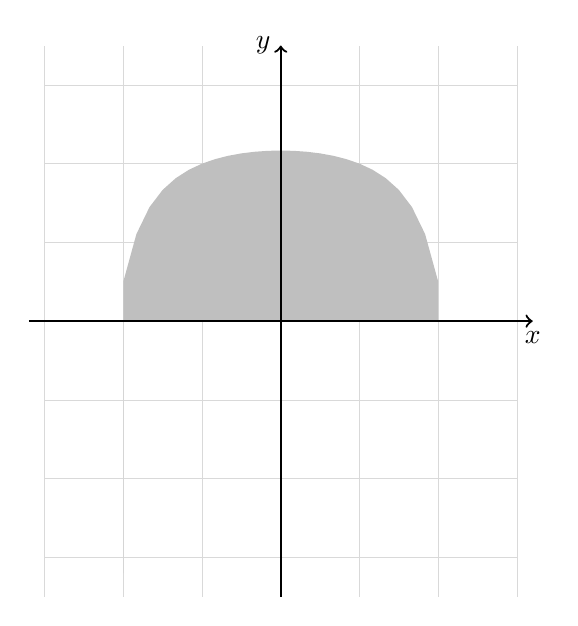
\begin{tikzpicture}
  
    \draw[very thin, gray!30, step = 1cm] (-3, -3.5) grid (3, 3.5);
    \fill[lightgray, domain = -2 : 2, variable = \x]
      (-2, -3.2)
      -- plot ({\x}, {(\x * \x - 1) / (\x * \x - 6) + 2})
      -- (2, 0)
      -- (-2, 0)
      -- cycle;
  
    \draw[thick] [->] (-3.2, 0) -- (3.2, 0) node[right, below] {\(x\)};
    \draw[thick] [->] (0, -3.5) -- (0, 3.5) node[above, left] {\(y\)};
  
  \end{tikzpicture}
  \caption{\(f(-x) = f(x)\)}\label{fig:int-symm-seg-even}
  \end{subfigure}
\end{figure}
